\documentclass{article}
\PassOptionsToPackage{dvipsnames}{xcolor}
\usepackage{arxiv}

\usepackage{algorithm}
\usepackage{algpseudocode}
\usepackage[utf8]{inputenc} % allow utf-8 input
\usepackage[T1]{fontenc}    % use 8-bit T1 fonts
\usepackage[hidelinks]{hyperref}       % hyperlinks
\usepackage{url}            % simple URL typesetting
\usepackage{booktabs}       % professional-quality tables
\usepackage{amsmath,amssymb,amsthm}
\usepackage{amsfonts}       % blackboard math symbols
\usepackage{nicefrac}       % compact symbols for 1/2, etc.
\usepackage{makecell}
\usepackage{microtype}      % microtypography
\usepackage{mathrsfs}
\usepackage{float}
\usepackage{graphicx}
\usepackage{doi}
\usepackage{acronym}
\usepackage{listings}
\usepackage{siunitx}
\usepackage{tabularx}
\usepackage{tikz}
\usepackage[dvipsnames]{xcolor}

\usetikzlibrary{trees}

\def\checkmark{\tikz\fill[scale=0.4](0,.35) -- (.25,0) -- (1,.7) -- (.25,.15) -- cycle;}
\def\cross{\tikz\draw[scale=0.3, black, line width=0.3mm](0,0) -- (1,1) -- (0.5,0.5) -- (0,1) -- (1,0) -- (0.5,0.5);}

\newacro{abm}[ABM]{Agent-Based Model}
\newacro{cabm}[CABM]{Cellular Agent-Based Model}
\newacro{ode}[ODE]{Ordinary Differential Equation}
\newacro{sde}[SDE]{Stochastic Differential Equation}
\newacro{pde}[PDE]{Partial Differential Equation}
\newacro{ca}[CA]{Cellular Automaton}
\newacro{ib}[IB]{Individual-Based}
\newacroplural{ca}[CA]{Cellular Automata}
\newacro{cpm}[CPM]{Cellular Pottes Model}
\newacro{ecoli}[\textit{E.coli}]{\textit{Escherichia coli}}
\newacro{bsubtilis}[\textit{B.subtilis}]{\textit{Bacillus subtilis}}
\newacro{paeruginosa}[\textit{P.aeruginosa}]{\textit{Pseudomonas aeruginosa}}
\newacro{pg}[PG]{peptidoglycan}
\newacro{a22}[A22]{S-(3,4-Dichlorobenzyl)isothiourea}
\newacro{mre}[\textit{mre}]{murein formation gene cluster E}
\newacro{tirf}[TIRF-M]{total internal reflection fluorescence microscopy}
\newacro{ecm}[ECM]{extracellular matrix}
\newacro{qs}[QS]{quorum sensing}
\newacro{crispr}[CRISPR]{Clustered Regularly Interspaced Short Palindromic Repeats)}
\newacro{flavo}[\textit{F. johnsoniae}]{\textit{Flavobacterium johnsoniae}}
\newacro{serratia}[\textit{S. marcescens}]{\textit{Serratia marcescens}}

\newcommand{\todo}[1]{\colorbox{WildStrawberry}{\textcolor{white}{#1}}}
\newcommand{\R}{\mathbb{R}}
\newcommand{\denovo}{\textit{de novo}}

\title{Spatial Models of Rod-Shaped Bacteria - Can AI link Single-Cell Essays and Collective Phenomena?}

%\date{September 9, 1985}    % Here you can change the date presented in the paper title
%\date{}                     % Or removing it

\author{
    \href{https://orcid.org/0009-0001-0613-7978}{
        \includegraphics[scale=0.06]{orcid.pdf}
        \hspace{1mm}Jonas Pleyer
    }
    \thanks{
        \href{https://jonas.pleyer.org}{jonas.pleyer.org},
        \href{https://cellular-raza.com}{cellular-raza.com}
    }\\
    Freiburg Center for Data-Analysis and Modeling\\
    University of Freiburg\\
    % \texttt{jonas.pleyer@fdm.uni-freiburg.de} \\
    \And
    \hspace{1mm}Toquinha-Orelia Bergmann\\
    Freiburg Center for Data-Analysis and Modeling\\
    University of Freiburg\\
    %% examples of more authors
    \And
    \href{https://orcid.org/0000-0002-6371-4495}{
        \includegraphics[scale=0.06]{orcid.pdf}
        \hspace{1mm}Christian Fleck
    }\\
    Freiburg Center for Data-Analysis and Modeling\\
    University of Freiburg
}

% Uncomment to remove the date
%\date{}

% Uncomment to override  the `A preprint' in the header
\renewcommand{\headeright}{Preprint}
%\renewcommand{\undertitle}{Technical Report}
\renewcommand{\shorttitle}{Spatial Models of Rod-shaped Bacteria}

\usepackage{enumitem}
\setlist{nolistsep}

%%% Add PDF metadata to help others organize their library
%%% Once the PDF is generated, you can check the metadata with
%%% $ pdfinfo template.pdf
\hypersetup{
pdftitle={Spatial Models of Rod-shaped Bacteria},
pdfsubject={q-bio.NC, q-bio.QM},
pdfauthor={Jonas Pleyer, Christian Fleck},
pdfkeywords={},
}

% Change numbering of equations
% \numberwithin{equation}{section}

\begin{document}
\maketitle

% TABLE OF CONTENTS
% Remove this before submission

%###################################################################################################
\begin{abstract}
    % \begin{itemize}
    %     \item Rod-shaped bacteria are everywhere
    %     \item many different species
    %     \item Shape plays crucial role in many effects such as motility, growth, collective effects etc.
    %     \item How does the behaviour of individual cells lead to collective phenomena?
    %     \item Mathemtical models help us to understand this
    %     \item We provide review of current state
    %     \item question; which biological required? answer: mesoscopic; want to get to emergent
    %         collective phenomena from single-cell behaviour
    % \end{itemize}
    Rod-shaped bacteria are ubiquitous forms of life which can be found in diverse microenvironments
    encompassing a wide, diverse range of species.
    Their elongated shape plays a crucial role in many biological processes such as enhancing
    swimming capabilities or promoting surface interactions.
    A key question is how the individual behaviour of multiple bacteria can lead to emergent
    spatial phenomena such as swarming and biofilm formation.
    Mathematical and computational methods provide powerful tools which allow researchers to bridge
    this gap and analyze the impact of various single-cell processes systematically.
    In this review we capture the current state of mathematical and computational approaches,
    emphasizing flexible, mesoscopic models which can be adjusted to describe a wide range of
    biological processes at their respectively required level of detail in order to study a variety
    of collective effects.
    We come to the conclusion that mechanical properties have been investigated extensively while
    other biolgical effects such as extracellular signalling, growth and differentiation are less
    studied.
\end{abstract}

% keywords can be removed
\keywords{Spatial \and Modeling \and Rod-Shaped \and Bacteria \and Mathematics}

% \textbf{POSSIBLE TITLES}
% \begin{itemize}
%     \item Mechanical Models of Rod-Shaped Bacteria - From Single-Cell Modeling to Collective Phenomena
%     \item Mathematical Modeling of Rod-Shaped Bacteria - From Single-Cell Mechanics to Collective Phenomena
%     \item Mathematical Models of Rod-Shaped Bacteria - From Single-Cell Analyses to Collective Phenomena
% \end{itemize}

\vfill
\pagebreak
\tableofcontents
\vfill
\pagebreak


%###################################################################################################
\section{Introduction}

\todo{move this to introduction}
Bacteria, unicellular divers procaryotic organisms and one of the simpler model to study individual single cell morphogenic changes up to emergent spatial emergent phenomena \cite{Vollmer2001}.
Various cell shapes are encountered in the prokaryotic world/Contain cells of different shapes, and yet we know little about how these shapes affect community biology \cite{Smith2017}.

Among the Well-studied examples include rod-shaped bacteria. Including gram negative as well as gram positive bacteria \ac{ecoli} (a Gram-negative bacterium) and \ac{bsubtilis} (Gram-positive) \cite{Chang2014}.

Including gram negative as well as gram positive bacteria \ac{ecoli} (a Gram-negative bacterium) and \ac{bsubtilis} (Gram-positive) \cite{Chang2014}.

\begin{itemize}
    \item Interested in all variations of rod-shaped bacteria; stiff, flexible, spiral, etc.
    \item Einordnung in andere Bakterienarten
    \item Rods are "more fundamtenal" than spheres (cocci) (which citation?)
    \item mesoscopic approach; take what cellular behaviour we need; interested in multicellular
        dynamics ultimately
    \item Talk about differences between: Gram-Positive, Gram-Negative
    \item Morphologies: Bacilli, Corkscrew, Filamentous, Spirochete
\end{itemize}

Order of this review
\begin{enumerate}
    \item Describe Biological Reality of Rod-shaped bacteria; single-cell; emergent phenomena
    \item What do we need within a model?
    \item Discuss modeling approaches; Mathematical, Computational
    \item Compare reusable computational tools
    \item Can we estimate their parameters?
\end{enumerate}

\section{Biological Functions}
\textbf{TODO Put a disclaimer here that says that we do not treat every aspect, but try to focus on
stuff which is important for us.}

\begin{enumerate}
    \item Cell wall and cytoskeleton fundamental as building blocks of cell shape
    \item How are they coupled?
    \item Describe mechanics of growth in rod-shaped bacteria
    \item How do single machineries regulate rod shape maintenance/shape?
    \item How does Division work?
    \item Brief outlook to other forms
\end{enumerate}

\begin{figure}
    \centering
    % 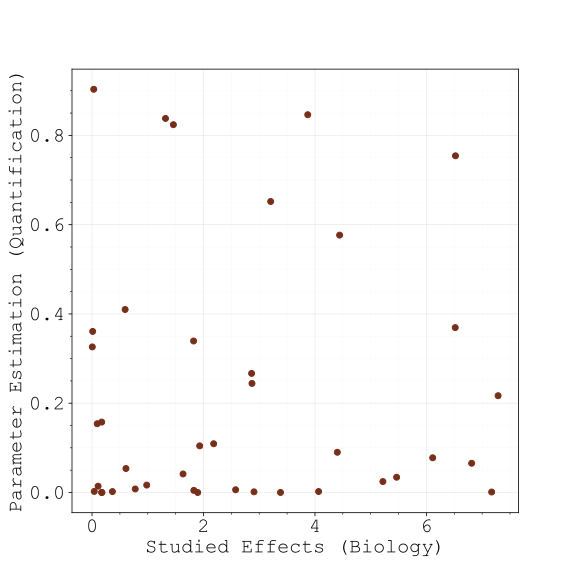
\includegraphics[width=0.5\textwidth]{figures/studies-scatterplots.pdf}%
    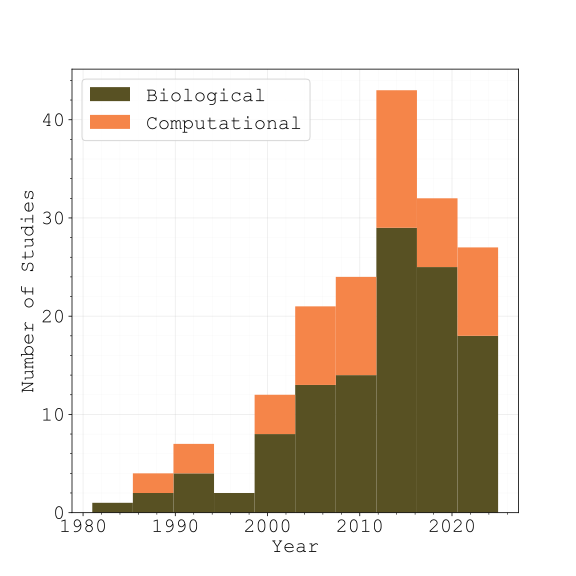
\includegraphics[width=0.5\textwidth]{figures/studies-over-time.pdf}
    \caption{
        TODO UPDATE FIGURES!
    }
\end{figure}

\subsection{Cell Wall, Cytoskeleton \& Interplay}
\textbf{This should be inserted somewhere}
\begin{itemize}
    \item \cite{Cylke2023} growth of \ac{ecoli} might be super-exponential; quantitative analysis of
        "morphogenetic noise"; interesting study about how the detailed mechanisms of growth in
        rod-like bacteria work
    \item \cite{Rosenberger1978} "Surface growth in rod-shaped bacteria" (Mathematical Model, model
        individual surface growth of one bacterium)
\end{itemize}

The shape of bacteria is mainly determined by their envelope and its growth. Most bacteria are surrounded by peptidoglycan \ac{pg}, a mesh-like macromolecule of glycan strands that are crosslinked via short peptides, which is chemically unique to bacteria~\cite{Cava2014, Amir2014, Cochrane2020}. This essential structure mechanically resists high turgor pressure, giving the cell its specific shape, isolating and regulating environmental uptake, which is indispensable for bacterial survival~\cite{Cochrane2020, vanTeeffelen2018}.

Although bacterial cell morphology is physically defined by \ac{pg}, an elongated shape requires cytoskeletal support. At the end of the last century, an actin-like protein MreB was discovered~\cite{Erickson2001}.  It's crystal structure \cite{Lowe2017_lj} and filament-forming dynamic \cite{Dersch2020} show strong similarity to actin. Additional actin-homologues, MreC, and MreD were later identified \cite{vandenEnt2001} playing an important role in shaping the cell.

MreB filaments make/form a spiral-like or banded pattern along the length of the cell, moving circumferentially around the lateral axis, coordinating \ac{pg} synthesis \cite{Garner2021, White2012, López2006}. Thus, MreB polymers' dynamics actively restrict and/or control the mobility of cell wall elongation complexes \cite{DEscobar2011}, thereby linking cytoskeletal organisation with local changes of cell shape \cite{Shi2018}. MreB filaments are attracted to regions of negative Gaussian curvature and excluded from regions of positive Gaussian curvature, such as the cell poles, thus driving maintenance of the shape \cite{vanTeeffelen2018, Olshausen2013}. The transmembrane protein, like RodZ, modulates MreB curvature preference \cite{Bratton2018}, altering MerB localisation and density.

\todo{Add Stiffness due to MreB here! "Counteracts curvature"}

\subsection{Growth, Maintenance \& Division}

Cell growth relies on the spatial and temporal regulation of \ac{pg} synthesis by different cytoskeletal molecules. The cell wall elongation is achieved by new \ac{pg} being inserted in discrete patches at the surface of the cytoplasmic membrane, a process coordinated by MreB and/or its homologues \cite{DePedro2003}. There are two growth mechanisms. During elongation, cells maintain a constant diameter \cite{Billaudeau2017}, expanding their surface area primarily along the sidewall. During constriction, polar \ac{pg} synthesis initiates the formation of new polar caps \cite{Cooper1991, Wang2010_2}. This process is comparable for both gram-negative and gram-positive bacteria, despite their varying wall thicknesses \cite{Chang2014}. However, species-specific differences in wall architecture and thickness influence elongation dynamics (for example, variations in \ac{pg} assembly patterns and machinery organisation lead to distinct elongation behaviors in \ac{bsubtilis} and \ac{ecoli}, as shown by  \cite{Billaudeau2017}). Most bacteria obtain their elongation through MreB-dependent lateral growth. In contrast, a few species lacking an MreB system elongate at the poles using division machinery that remains active after division/constriction \cite{Daniel2003}. 

Despite growing, the cell must actively maintain its shape. Cell shape is balanced by two processes: wall elongation and septum formation. A lack of elongation due to evolution or mutation results in cocci-shaped cells \cite{Lleo1990}. Consistently, ac{mre} mutants \cite{Wachi1987}, \textit{rodZ} deletion mutants \cite{Shiomi2008}, as well as cells treated with \ac{a22} \cite{IWAI2002}, which disrupts MreB assembly \cite{Bean2009}, were found to cause spherical cell shape. This indicates that cell shape. This indicates that cell shape maintenance involves proteins encoded by the \ac{mre}  genes, such as MreB, or proteins that interact with them.
Furthermore, \cite{Jones2001}  showed that MreB regulates cell width, whereas Mbl controls linear axis regulation. MreB filaments move circumferentially around rods of any width; however, filament motion is isotropic in spherical cells, moving in all directions \cite{Garner2021}. Highlighting the fact that the regulation of geometry by the cytoskeleton extends beyond elogated-shaped bacteria.
Finally, a switch in, or de novo, \ac{pg} synthesis is sufficient to regenerate the cell wall and restore the original shaped morphology, both in spherical cells \cite{Huan2021} and in L-forms \cite{Kawai2014}.

Bacterial morphogenesis is plastic and can be reprogrammed to change the growth and division axis \cite{denBlaauwen2018}.  \cite{Takeuchi2005} experimentally altered \ac{ecoli} morphologies without modifying any additional biochemical or genetic functions and thereby automatically altered cell motility, suggesting that cell shape is an evolutionary trait influencing nutrient uptake, cell division and segregation, adhesion, passive and active motility, predator avoidance, and cellular differentiation \cite{Young2006}. \cite{Young2006} also suggested that the earliest cells consisted of rods and filaments, with cocci being less common. More complex shapes oftenrequire distinct or additional cell-wall-machineries \cite{Zapun2008} or cytoskeletal components like crescentin the bacterial equivalent of intermediate filaments (IFs)\cite{Ausmees2003}. This hints that in the absence of an active, MreB-dependent shape-determining system, the default shape is spherical \cite{Jones2001}, whereas rod shape represents the simplest morphology mediated by \textit{mreB} systems.

Cell division is inhibited by two systems: the Min system, which prevents division near the cell poles, and nucleoid occlusion, which prevents cell division over nucleoids  \cite{Bramkamp2009, Oliva2004}. When both systems are inactivated, FtsZ assembles to form a central ring (Z-ring), generating the constriction forces required for division \cite{Li2007}. 
Beyond these regulatory systems, morphogenesis and \ac{pg} synthesis are mechanically sensitive, indicating that growth patterns are adaptive and coupled to physical forces \cite{Si2015}. The division site is favored by these mechanical forces \cite{Li2007, Koch1995, Chatterjee1988}. Furthermore, the division trigger itself, particularly in \ac{ecoli}, is regulated by size-sensing mechanisms rather than a strict timing mechanism \cite{Robert2014}, and spatial variation of mechanical stress in the cell also contributes to growth patterns, shape maintenance, and division site selection \cite{Chatterjee1988}.
The Z-ring tension regulates \ac{pg} synthesis \cite{Lan2007}, switching it from dispersed insertion to a concentrated local mode for new synthesis at the cell poles \cite{DenBlaauwen2008}. Additionally, the surface synthesis rate increases, supporting the idea of separate elongation and division machineries  \cite{Woldringh1987, Cooper1991}. In terms of physical properties, MreB and \ac{pg} contribute to nearly equal parts to the stiffness of a cell \cite{Wang2010, Wang2010_protocol}. Furthermore, MreB contributes to the formation of a bacterial mitotic-like machine and controls bacterial DNA segregation  \cite{Kruse2005, Gitai2005}.
However, segregation of the origin region is unaffected by \ac{a22} treatment \cite{Karczmarek2007} highlighting complexity in MreB's function. Finally, despite symmetric division, aging and mortality can occur through the asymmetric inheritance of cellular damage (the older 'mother' cell poles accumulate damage or growth defects over generations) \cite{Stewart2005}.


\subsection{Reaction to Environmental Factors}
Bacteria continuously sense, interpret and respond to environmental cues through a variety of physical, biochemical and behavioural mechanisms.
One fundamental behavioral mechanism is taxis, which is highly adapted to the species' environment. It enables the integration of multiple diverse external stimuli, such as chemicals (chemotaxis), light (phototaxis), oxygen (aerotaxis), temperature (thermotaxis), and magnetic fields (magnetotaxis). Hence, it allows for species-specific and highly adapted navigation strategies \cite{Krell2011}. Of these, chemotaxis is one of the most common and best studied. It is a receptor-mediated signalling network that integrates external chemical cues to controlling movement direction \cite{Nikita2009, Bourret2002}.

Guiding cells away from harmful conditions to more survival-friendly habitats, linking environmental sensing to regulation of cellular metabolism and nutrient acquisition. Metabolism is thus central to survival, driving nutrient uptake which is mediated by highly selective transporter systems (e.g., ABC transporters, TRAP systems, and PTS) that import sugars, amino acids, ions, carbon, nitrogen, iron, and lipids...... Bacteria can also modulate cell envelope permeability and secrete enzymes to facilitate nutrient acquisition \cite{Davies2021, Niederweis2008, Tanaka2018, Li2025}.
Significant nutrient uptake can dissolve inorganic sources and modify the cell environment, competing with other microorganisms \cite{Caron1994}. Additionally, a diverse part of bacteria are predators and found in various environments, shaping microbial community structure and dynamics, through distinct predatory strategies with independent evolutionary origins \cite{Velicer2009, Rory2015}. 
Motile chemotactic bacteria have an enhanced nutrient uptake rate compared to non-motile cells \cite{Watteaux2015}, highlighting the importance of movement and adherence in competitive and challenging environments.

Bacteria employ different modes of motion depending on their morphology and appendages.
Swimming cells are short, mononucleate, flagellated for planktonic motility \cite{Alberti1990}. The swimming motion of bacteria is regulated by shape and taxis \cite{Kong2014}, and the bending stiffness of the flagellar filament supports propulsion and reorientation during swimming, which remains constant over time \cite{Shen2022}. Most of the swimmers can differentiate into swarmer cells when growing on surfaces, increasing in cell length and number of flagella per cell \cite{Alberti1990, Harshey1994}. 
Swarming, in contrast to the directed, single-cell movement of swimming, is a collective behavior in which individual cells suppress chemotaxis and instead exploit the dynamics of the group to continuously expand and acquire new territory \cite{Harshey2015, Kearns2010}.
Twitching represents another form of appendage-generated movement. A Type IV pili generate retraction forces, pulling the cell across surfaces \cite{Chang2016}, and the non-Newtonian behavior of extracellular slime further enhances gliding by optimizing force transmission and energy use \cite{Shah2022}.
Gliding is a flagella-independent mode of surface motility, relying on an outer-membrane complex that attaches to the substrate at fixed focal adhesion sites, enabling directional movement \cite{ContrerasM2024, Shrivastava2015}.
Sliding describes passive surface spreading driven by cell growth and surfactant-mediated surface tension reduction rather than active appendage-based motility \cite{Kearns2010}.

Cell appendages, in addition, are not only used for locomotion. Type IV pili \cite{Ellison2021, Maier2015} or flagella in general \cite{Haiko2013} are more than force-generating structures that coordinate bacterial movement; they also play an important role in adhesion and environmental interaction. This is mainly driven by physicochemical interactions: van der Waals, electrostatic, hydrophobic, and acid-base forces, whose strength is determined by the surface properties (charge, hydrophobicity, roughness) \cite{vanLoosdrecht1989, Hori2010}. It is a highly heterogeneous and dynamic process mediated by additional surface structures e.g. adhesins, fimbriae, cadherins and other surface proteins, allowing specific binding to \ac{ecm} components \cite{BrettFinlay2014, Berne2018} attachment to a host \cite{Beachey1981, Vaca2019}, formation of mechanical links between neighboring cells \cite{Whitfield2006} or pulling cells together and promoting microcolony formation \cite{Ellison2021}. In some rare cases, bacteria can fuse when they remain in close proximity for extended periods \cite{Kudryashev2011}.

Beyond environmental sensing and movement, bacterial survival also depends on adaptive responses to changing conditions. When encountering new nutrients, bacteria enter a lag phase. An adaptive phase in which there is no division. During this dormant stage, metabolic adaptation and macromolecular synthesis occur to prepare for rapid cell growth and robust cell division \cite{Bertrand2019}. This response is heterogeneous and asynchronous, providing it an adaptive advantage \cite{Senkei2007}. Additionally, under acute stress, some cells can enter a non-replicating, deep dormant state known as persistence. These persister cells play a central role in surviving infectious disease or antibiotic treatment, notably achieving survival without requiring genetic resistance or permanent adaptation \cite{Wood2013, Lewis2006}.
In parallel with these dormant strategies, bacteria have evolved an adaptive resistance mechanism against bacteriophages \ac{crispr} \cite{Duckworth2002, Barrangou2007} (\cite{Borges2017} some protein families have anti-CRISPR function).Crucially, the rapid accumulation and sharing of such adaptive traits, including resistance and metabolic capabilities, are achieved via bacterial conjugation. A key mechanism for horizontal gene transfer, enabling bacterial communities to adapt collectively and maintain functional diversity \cite{Virolle2020, Kong2018}.


\subsection{Living as a Community}
While living in a dense community, crowding and cell-cell forces act together to constrain growth, linking intracellular density with external mechanical stress \cite{Alric2022}. These mechanical interactions can reshape cellular behaviour and gradients, enabling long-term adaptive diversification \cite{Badyaev2025}. Such physically constrained environments necessitate robust chemical communication. Alongside this mechanical collective response, bacteria produce and secrete small signalling molecules called autoinducers, a process known as \ac{qs}. \ac{qs} enables cells to coordinate collective gene expression and adaptive group behaviour once the autoinducer reaches a critical threshold concentration. Thereby, processing information at the population level and enhancing decision-making accuracy through coordinated responses \cite{Stephen2007, MorenoGmez2023}. \ac{qs} acts as a population-level decision system that links survival and programmed cell death, using selective lysis to strengthen biofilm structure and thereby optimize collective fitness \cite{Leung2015, Senadheera2008, Dufour2013, Mashruwala2024}. \ac{qs} does not only mediate communication within a single species; it also mediates communication between species and across kingdoms, such as in bacteria-host or bacteria-virus systems. \cite{Hense2007, Boyer2009, Liu2025}. It is a key mechanism in mature biofilms for coordinating differentiation, for example, enabling transition from a sessile community to a free-living state \cite{Solano2014}.

Bacteria have adapted a variety of multicellular strategies to survive in a community. One previously mentioned example is the swarming cell, which is a long, multinucleate, hyperflagellated bacterial cell that enables active and rapid surface motility. In this state, cells exhibit increased resistance to multiple antibiotics \cite{Kim2003, Lai2009}. Other forms of differentiation like cellular specialization including the distinction between matrix producers and surfactant-producing cells, serve to stabilize and coordinate the colony structure \cite{Lopez2010, Flemming2016}.
Beyond active specialization, many bacteria employ sporulation as a survival strategy under harsh environmental conditions. When these spores germinate, they restore vegetative morphology \cite{Huan2021, Errington2020, Licking2000, Barák2019, Jose2016, Branda2001}. The sporulation process itself is highly individual for the species. Some bacteria have starvation-dependent and starvation-independent pathways \cite{Licking2000}, while others can divide asymmetrically during sporulation \cite{Barák2019}. Some bacteria have developed even more complex life cycles, leading to the formation of fruiting bodies. These are multicellular aggregations of differentiated cells where spore formation is favored \cite{Licking2000, Jose2016, Branda2001}.

Together, these multicellular behaviors contribute to the emergent lifestyle observed in biofilms.
Adhesion is the fundamental phenomenon that drives the initial colonization and persistence of bacteria on diverse surfaces \cite{Dunne2002, Ong1999, vanLoosdrecht1989, Hori2010}. This process is determined both by bacterial features and the properties of the respective biomaterial.
Subsequently, competition for surface colonization drives specific strategies that target adhesion, signaling, and matrix dynamics. This allows mixed-species biofilms to regulate neighbor entry and, consequently, the internal community structure \cite{Rendueles2012}.
As growth progresses, expanding colonies are further organized by collective motility and chemotactic interactions. This manifests, for example, in swarming-driven branching and the formation of vortex-like patterns \cite{Ingham2008}. Beyond collective motility, the mechanical properties of the cell and their extracellular matrix can impose large-scale structures, such as wrinkled pellicles formed by matrix elasticity \cite{Trejo2013}. The division of labor additionally contributes to spatial colony self-organization. Examples include matrix-producers forming aligned bundles (“van Gogh bundles”) whose physical properties set the expansion rate of the colony and surfactin-producers reduce surface friction \cite{Li2025, vanGestel2015, Lopez2010, Flemming2016}. This mechanical organization also supports colony structure robustness, enabling self-healing by reconnecting or regrowing structural bundles \cite{Dong2022}. Moreover, confinement and mechanical forces drive the transition of biofilms from 2D to 3D structures. This process is dependent on cell elasticity, elastic interactions, and friction between bacteria and the surrounding medium \cite{Duvernoy2018, Grant2014}.
Despite the strong competition, biofilms represent a favored lifestyle as they offer critical survival advantages. A core benefit is enhanced survival and stress tolerance. Even when densely packed, the three-dimensional biofilm growth and matrix architecture facilitate the collective capture of resources. \cite{Nadell2017, Arjes2021}. 
Additionally, in mixed-species biofilms, antimicrobial-resistant keystone species mediate the survival \cite{Wisnu2022, Flemming2016}


\subsubsection{Spatial Organization - Modelling papers remaining}
\begin{itemize}
    \item \cite{Starru2007} while non-chemical, physical cell-cell interactions drive emergent collective motion patterns such as vortices and streams. Cell shape as the length-to-width ratio controls the level of clustering thereby strongly influencing swarm dynamics. \todo{WRONG CITATION HERE?}
    \item \cite{Jin2020,Jin2020_2} adhesion, friction, and cell stiffness influence colony morphology- stronger cell-cell adhesion leads to denser, slower-growing biofilms, while weaker adhesion promotes faster spreading
    \item \cite{Li2025} AGB modeling \cite{vanGestel2015} biological properties already mentioned
    \item \cite{Buka1987} "For example, injection of a flux of a liquid crystal between two close parallel plates (viscous fingering) causes orientation of the molecules to couple with the flow, with the resulting emergence of dendritic patterns." (Wikipedia) \todo{put this into "active matter" section?}
\end{itemize}


\section{Mathematical \& Computational Frameworks}
\subsection{Active Matter as a Continuum}
\textbf{keywords:}
filamentous, nematic order

\begin{itemize}
    \item \cite{Duman2018} "Collective dynamics of self-propelled semiflexible filaments"
        (no division, no intracellular dynamics, no growth)
    \item \cite{Joshi2019} "The interplay between activity and filament flexibility determines the
        emergent properties of active nematics"
    \item \cite{Modica2024} "Soft confinement of self-propelled rods: simulation and theory"
    \item \cite{Peruani2006} "Nonequilibrium clustering of self-propelled rods"
    \item \cite{Saintillan2013} "Active suspensions and their nonlinear models" (suspensions of
        self-propelled microorganisms, dynamics of chemotactically responsive)
    \item \cite{Wensink2012} "Meso-scale turbulence in living fluids" (contains coarse-graining)
    \item \textbf{TODO look for more mixed-morphology (rods \& spheres) papers}
    \item BacSim-T6SS~\cite{Lin2023} "A subcellular biochemical model for T6SS dynamics reveals winning competitive strategies"
    \item \cite{Boyer2011} "Buckling instability in ordered bacterial colonies"
    \item \cite{Volfson2008} TODO; continuum model, equations of nematodynamics \cite{Doi1988-ad}
    \begin{align}
        \partial_t \rho + \partial_z (\rho \nu) &= \alpha \rho\\
        \partial_t q + \nu \partial_z q &= B(1-q^2) \partial_z \nu\\
        \partial_t(\rho \nu) + \nu \partial_z (\rho \nu) &= - \partial_z p - \mu \rho \nu
    \end{align}
    \item \cite{You2018} Hard-Rod model, continuous model
    \begin{itemize}
        \item shows how single-cell model can be translated into continuum model in large-scale edge
            case
    \end{itemize}
    \item \cite{Schwarzendahl2022} "Do active nematic self-mixing dynamics help growing bacterial colonies to maintain local genetic diversity?"
    \item \cite{Moreau2018} theoretical study abut asymptotic coarse-graining model for slender rods, biofilaments, and flagella
\end{itemize}

\subsection{Swimming}
\begin{itemize}
    \item \cite{Hsu2009} "A 3D Motile Rod-Shaped Monotrichous Bacterial Model" (Mathematical \&
        Numerical model for cylindrical (rigid) rods which move with flagella)
    \item \cite{Hu2015} "swimming properties of an E. coli-type model bacterium are investigated by
        mesoscale hydrodynamic simulations"
    \item \cite{Cooper2006} "we conjecture that the current observed shape of these bacteria may
        have been determined, in part, to obtain the most efficient shape for moving through liquids."
    \item \cite{Schuech2019} study movement of cells in liquid; curvature vs elongation; take into account curvature; have in-silico model
\end{itemize}

\subsection{Individual-based Models}
\textbf{Further studies with \ac{abm} and rod-shaped bacteria}
\begin{itemize}
    \item \cite{Winkle2017} "Modeling mechanical interactions in growing populations of rod-shaped bacteria" \textit{only "stiff" bacteria, growth inside mother machine}
    \item \cite{Winkle2021} "Emergent spatiotemporal population dynamics with cell-length control of synthetic microbial consortia" \textit{this continues the publication before, also has lattice-based model}
    \item \cite{Doumic2020} "A purely mechanical model with asymmetric features for early morphogenesis of rod-shaped bacteria micro-colony" \textit{"stiff" bacteria with overlaps, does some parameter estimation}
    \begin{itemize}
        \item This is a really good paper for referencing
        \item no bending in mathematical model
        \item Compare distributions of "Read-Outs" to data
        \item uses steric force (see also previously \cite{Trejo2013})
    \end{itemize}
    \item \cite{Grant2014} purposely-built model written in `C++`
    \begin{itemize}
        \item describes bacteria as collection of overlapping spheres
        \item spheres are coupled by non-linear springs (Euler-Bernoulli dynamic beam theory);
        This assumption is unfounded; they show however that it does not alter their results in this
        case
        \item only model repulsive forces; no attraction, adhesion
        \item investigate transition from 2D to 3D colony
    \end{itemize}
    \item \cite{Cho2007} only 2D, no bending, no parameter estimation; based on work done in 
        \cite{Jnsson2005}
    \item \cite{Storck2014} TODO;
    41 Parameters for various cases;
    only 8 parameters taken from literature values/quantified;
    generated growth rate randomly (normal distribution), but for each growth step; this is
      stochastically equivalent but numerically slightly more intense;
    \item \cite{Kong2014} TODO "Swimming motion of rod-shaped magnetotactic bacteria: the effects of
        shape and growing magnetic moment"
    \begin{itemize}
        \item single-cell study
        \item magnetotactic bacterium, swimming in viscuous liquid
    \end{itemize}
    \item \cite{Constantino2016} "Helical and rod-shaped bacteria swim in helical trajectories with
        little additional propulsion from helical shape"
    \begin{itemize}
        \item single-cell study
    \end{itemize}
    \item \cite{Starru2007} TODO very interesting FEM-based model
    \begin{itemize}
        \item single-cell study
        \item has on-lattice and off-lattice approach
        \item has bending of cells
        \item also shows some type of vortex formation
    \end{itemize}
    \item \cite{Valdez2025} "Biomechanical modeling of spatiotemporal bacteria-phage competition"
\end{itemize}

\subsubsection{Why ABMs are THE tool}
\begin{itemize}
    \item \cite{Nagarajan2022} Agent-Based Modeling of Microbial Communities \todo{use contents of this review}
\end{itemize}

Since the beginning of this decade, multiple tools have emerged which are able to describe living
systems on a cellular individual-based approach in various details.
A good reason for choosing a framework over a purpose-built solution is to follow the Findability,
Accessibility, Interoperability and Reuse) FAIR principles by \cite{Wilkinson2016}.
These criteria have been designed to improve the overall infrastructure surrounding (re)usability of
scholarly data and methods.
In our previous work, we investigated their differences and features and capacity to model
individual behaviour of cells \cite{Pleyer2023}.
Using one of these existing toolkits means that already existing functionality can be used to
develop own models and the produced research results can be fed back to the library for fellow
researchers to reuse.
This begs the question, which of these existing models is able to support the long list of aspects
that we set out to describe with the experimentally gathered evidence.

\textbf{TODO Include them}
\begin{itemize}
    \item \cite{Abar2017} "Agent Based Modelling and Simulation tools: A review of the state-of-art software"
    \item other generic frameworks exist, which may allow to model the desired functions
    \item \cite{Grimm2006,Grimm2010} \textbf{TODO} "A standard protocol for describing individual-based and
        agent-based models" and update: \cite{Jang2012}
\end{itemize}

\subsubsection{The Geometric Challenge (rename this)}
\paragraph{To Rod .. or not to Rod}

\begin{itemize}
    \item \cite{Ghaffarizadeh2018} PhysiCell; no rods
    \item \cite{Swat2012} CompuCell; uses \ac{cpm}; no rods
    \item \cite{Cooper2020} Chaste; cell-centre and vertex-based; no rods
    \item \cite{Starru2014} Morpheus, uses \ac{cpm}; no rods
    \item \cite{Wei2013} BNSim; cells are spheres
    \item \cite{Kreft1998,Kreft2001,Lin2023} (BacSim) "Individual-based modelling of biofilms Free"
    \item \cite{Wei2013} BNSim; cells are spheres
    \item \cite{Li2019} NUFEB \textbf{TODO}
    \item \cite{Hoehme2010} Tisim/CellSys \textbf{TODO}
    \item AgentCell~\cite{Emonet2005} no rods
    \item COMETS~\cite{Harcombe2014} grid-based approach
    \item McComedy~\cite{Bogdanowski2022} only spherical
    \item MultiCellSim~\cite{Dang2020} only lattice points (or spheres depending on interpretation)
    \item Netlogo~\cite{Banitz2015,vanderWal2013} very generalized \ac{abm}, not particular for biology (citations are only for specific applications, not Netlogo itself)
    \item NUFEB~\cite{Li2019} only soft spheres
\end{itemize}

Of the most popular frameworks, most do not support rod-shaped bacteria out of the box.
The very popular Cellular Potts Model (CPM) \cite{Graner1992} is mostly applied in 2D and only
represents cells as lattice grid points.
Since CompuCell3D \cite{Swat2012} exclusively builds upon the CPM, it can not model rod-shaped
bacteria.
PhysiCell \cite{Ghaffarizadeh2018} was designed to answer questions surrounding cancer research and
currently only supports spherical agents.
Chaste \cite{Cooper2020} was also designed for cancer research but further targets the heart and
tissues.
Naturally its Agent-Based Model supports cell-centre and vertex-based models but no rod shapes.
Morpheus \cite{Starru2014} also employs the CPM along with other spatial representations such as
vertex-based models or PDEs but has no support for Rod-Shaped bacteria.
Even purpose-built solutions such as BNSim \cite{Wei2013} which specifically targets bacterial
networks, assumes a simplified spherical representation for their bacterial agents.


\subsubsection{Integrated Modeling Tools}
\paragraph{With Rods (check and mention them)}
\begin{itemize}
    \item \cite{Breitwieser2021,breitwieser_biodynamo_2022} BioDynamo, cylinders
    \item \cite{Gorochowski2012,Matyjaszkiewicz2017} BSim; has rods
    \item \cite{Kang2014} (Biocellion) only cylindrically-shaped potentials
    \item \cite{Gutirrez2017} \texttt{gro} only rods
    \item \cite{Pleyer2025} \texttt{cellular\_raza} flexible rods
    \item \cite{Lardon2011} iDynomics
    \item \cite{GoiMoreno2015} DiSCUS cylinders
    \item \cite{Rudge2012} CellModeller, has rod-shaped support and some predefined chemical reactions etc.
\end{itemize}

As we have seen, many frameworks do not provide existing functionality for rod-shaped bacteria.
However, some others do have various levels of support.
Biocellion \cite{Kang2014} can model agents with cylindrical interaction potentials but does not
model any of the MreB-related bending and rigidity or polar interactions.
They acknowledge this shortcoming: "Mapping a cell to multiple agents is also necessary to
separately model subcellular compartments [..].
However, Biocellion does not yet support this." \cite{Kang2014}
BSim2.0 represents cells as rigid capsular cells made from a cylindrical center part and two
half-spheres, which are placed at the ends of the cylinder to round out the shape.
In order to calculate interactions between cells, possible overlaps are determined and minimized,
thus determining the position values of the next iteration step.
It also accounts for many other phenomena, which are displayed in \textbf{TODO replace}.
BSim does not consider bending forces for individual cells or polar interactions.
The \texttt{gro} programming language was designed to simulate the growth of colonies and cell-cell
communication.
Its "physics computation has been optimized for rigid rod-shaped bodies, like E. coli bacteria"
\cite{Gutirrez2017}.
They recognize two types of forces which are acting on the cellular agents:
\textit{Local forces} which are calculated between adjacent bacteria and a \textit{global force}
which pushes bacteria outwards of the colony.
The latter of these is a phenomenological implementation of the observed colony expansion and the
associated central pressure with it.
This assumption may yield incorrect results for sparsely populated cases.
The engine is limited to 2D and does not consider polar interactions or bending of the rods.

\begin{table}
    \centering
    \textbf{Only include frameworks if they have rods}\\
    \begin{tabularx}{\textwidth}{lccccccccc}
        \toprule
        Name & Shapes & Intra & Extra & Motility & Chemotaxis & Ext. Forces & Dim & Date\\
        \midrule
        % BacSim~\cite{Kreft1998,Kreft2001} & S & Fix & Diff & - & - & - & 2 & 1998\\
        % BNSim~\cite{Wei2013} & S & O,So & Diff & R & \checkmark & - & 3 & 2013\\
        Biocellion~\cite{Kang2014} & S,C & Discr & R,Diff & R & - & - & 3 & 2014\\
        BioDynamo~\cite{breitwieser_biodynamo_2022} & S,C & O,U & Diff & R,U & \checkmark & - & 3 & 2022\\
        BSim~\cite{Gorochowski2012,Matyjaszkiewicz2017} & C & O & Diff & R & - & - & 2,3 & 2013\\
        \texttt{cellular\_raza}~\cite{Pleyer2025} & S,C,F,U & O,U & Diff,U & R,U & U & U & 2,3 & 2025\\
        CellModeller~\cite{Rudge2012} & C & O,Discr & Diff & - & - & F & 3 & 2012\\
        % has rod-shaped support and some predefined chemical reactions etc.\\
        DiSCUS~\cite{GoiMoreno2015} & C & O & - & - & - & - & 2 & 2015\\
        \texttt{gro}~\cite{Gutirrez2017} & C & O & Diff & - & - & - & 2 & 2017\\
        iDynomics~\cite{Lardon2011} & S,C & O & Diff & - & - & F & 2,3 & 2011\\
        Tisim/CellSys~\cite{Hoehme2010} & S & O & Diff & R & - & - & 2,3 & 2010\\
        \bottomrule
    \end{tabularx}
    \begin{minipage}{0.4\textwidth}
        \caption{Overview of modeling frameworks with varying support for cellular and environmental
        aspects.}
    \end{minipage}%
    \begin{minipage}{0.6\textwidth}
        \begin{tabularx}{\textwidth}{ll}
            \textbf{Legend}\\
            \midrule
            Cell shapes & (S) Spherical, (C) Cylindrical, (F) Flexible\\
            Intracellular & (O) \acp{ode}/\acp{sde}, (Discr) Discrete\\
            Extracellular & (R) Reactions, (Diff) Diffusion\\
            Motility & (R) Random/Stochastic Motion\\
            External Forces & (F) Fluid/Flow\\
            Other & (U) User definable\\
            \bottomrule
        \end{tabularx}
    \end{minipage}%
\end{table}

\section{Common Building Blocks (Behaviour)}
\begin{itemize}
    \item aspect groups (C), (CC), (CE) are related to computational approaches\\
        for c in cells\\
        for c1 in cells: for c2 in cells: calculate\_interaction(c1, c2);\\
        for c in cells; interact\_with\_domain(c, domain);
    \item summarize what we have learned from biology and from computational approaches
    \item identify common subgroups, called aspects that are shared between the various models
    \item building blocks in nature:
        physical entities (objects of physical extension),
        in software: behaviour (components which describe effects)
\end{itemize}

\subsection{Computational Abstractions}


\ref{algorithm:generalized-main-loop}
\ref{fig:concept-figure-aspects}

\begin{algorithm}
    \caption{Schematic Main Loop of Simulation Frameworks}
    \label{algorithm:generalized-main-loop}
    \begin{algorithmic}[1]
        \Procedure{main\_loop}{$t_0$, $t_\text{max}$, $\Delta t$}
        \State \texttt{cells} $\gets$ \texttt{initialize\_agents()} \Comment{Define initial state}
        \State \texttt{$\mathscr{E}$} $\gets$ \texttt{initialize\_environment()}
        \State $t\gets t_0$
        \While{$t<t_\text{max}$}
            \For{$c$ in \texttt{cells}} \Comment{(C) Cellular}
                \State \texttt{update\_internal\_states}($c, t, \Delta t$)
            \EndFor
            \State \texttt{interacting\_cells} $\gets$ \texttt{determine\_interacting\_cells(cells)}
            \For{$c_1,c_2$ in \texttt{interacting\_cells}} \Comment{(CC) Cell-Cell}
                \State \texttt{perform\_interaction}($c_1, c_2, t, \Delta t$)
            \EndFor
            \For{$c$ in \texttt{cells}}
                \State \texttt{react\_to\_environment}($c$, $\mathscr{E}, t, \Delta t$) \Comment{(CE) Cell-Environment}
            \EndFor
            \State \texttt{update\_environment}($\mathscr{E}, t, \Delta t$) \Comment{(E) Environment}
            \State $t\gets t + \Delta t$ \Comment{Increment Time}
        \EndWhile
        \EndProcedure
    \end{algorithmic}
\end{algorithm}

\begin{figure}
    \centering
    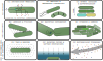
\includegraphics[width=\textwidth]{figures/concept-figure-2.png}
    % \includegraphics[width=\textwidth]{figures/gemini-concept-figure.pdf}
    % 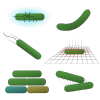
\includegraphics[width=0.5\textwidth]{figures/concept-figure.png}
    % \includegraphics[width=0.2\textwidth]{figures/41579_2010_Article_BFnrmicro2405_Fig1_HTML.pdf}
    \caption{
        \textbf{TODO}
        % \todo{\cite{Kearns2010} fig. 1. good movement review, maybe include figure}
    }
    \label{fig:concept-figure-aspects}
\end{figure}

\begin{itemize}
    \item biological phenomena have been summarized before
    \item emphasize: more than just mechanics, also incorporate cell-cycle, extracellular
        reactions, (polar) interactions, etc.
    \item present "grouping" of biological phenomena into: (C) Cellular, (CC) Cell-Cell, (DC)
        Domain-Cell aspects \textbf{TODO possibly rename Domain to Environment}
    \item explain aspect-groups
    \item discuss table \ref{table:simulation-aspects}
\end{itemize}


\begin{table}[H]
    \newcounter{aspect}
    \setcounter{aspect}{1}
    \newcommand{\asp}{(\arabic{aspect}\refstepcounter{aspect})}
    \centering
    \def\arraystretch{1.3}
    \begin{tabularx}{\textwidth}{c l X}
        &\textbf{Aspect} & \textbf{Details \& Examples}\\
        \toprule
        &\multicolumn{2}{l}{\textbf{(C) Cellular}}\\
        \midrule
        \asp & Shape & Cell Wall~\cite{Cava2014, Amir2014, Cochrane2020}, Cytoskeleton~\cite{Erickson2001,Dersch2020}, Maintenance~\cite{Billaudeau2017}, Stiffness~\cite{Wang2010, Wang2010_protocol,Takeuchi2005,Ursell2014,Amir2014_2}\\
        \asp & Growth & Lag-phase~\cite{Senkei2007, Bertrand2019}, Polar/Lateral Elongation~\cite{Robert2014,Takeuchi2005,Daniel2003,Cooper1991, Wang2010_2}, Dormancy \cite{Wood2013,Lewis2006} \\
        \asp & Movement & Swimming~\cite{Alberti1990,Kong2014}, Gliding~\cite{ContrerasM2024, Shrivastava2015}, Sliding, Directed, Stochastic, Appendages (flagella, pili)\\
        \asp & Reactions & Gene-Regulatory Networks\cite{Duckworth2002, Barrangou2007}, Metabolism~\cite{Davies2021, Niederweis2008, Tanaka2018, Li2025}\\
        \asp & Division~\cite{Bramkamp2009, Oliva2004} & Asymmetric~\cite{Stewart2005}, Z-Ring~\cite{Li2007}, Inheritance of Properties ~\cite{Robert2014}\\
        \asp & Differentiation & Matrix-producing, surfactin-producing~\cite{vanGestel2015,Lopez2010}, Sporilation~\cite{Licking2000,Barák2019}, Fruiting Bodies~\cite{Licking2000, Jose2016, Branda2001}\\
        \asp & Death & - \ac{qs}~\cite{Leung2015, Senadheera2008, Dufour2013, Mashruwala2024}\\
        &\multicolumn{2}{l}{\textbf{(CC) Cell-Cell Interactions}}\\
        \midrule
        \asp & Short-Range Physical & Adhesion~\cite{Verwey1947,Trejo2013}, Friction~\cite{Doumic2020,Grant2014}, Volumetric Exclusion\\
        \asp & Long-Range Physical & Attraction, Polar Forces~\cite{Duvernoy2018}\\
        \asp & Contact Reactions & Bacterial Conjugation~\cite{Virolle2020, Kong2018}\\
        \asp & Neighbor Response & Crowding, Jamming\\
        &\multicolumn{2}{l}{\textbf{(EC) Environment-Cell Interactions}}\\
        \midrule
        \asp & Exchange of compounds & Uptake, Secretion~\cite{Li2025}, \ac{qs}~\cite{Stephen2007, MorenoGmez2023}\\
        \asp & Taxi/Sensing & Chemotaxis, Phototaxis, Thermotaxis, Magnetotaxis, Aerotaxis~\cite{Krell2011}\\
        \asp & External Forces & Fluidic forces~\cite{Amir2014_2}, Buyoancy, Stoke's, Gel~\cite{Grant2014}\\
        \asp & Surface Interactions & Adhesion~\cite{vanLoosdrecht1989}\\
        &\multicolumn{2}{l}{\textbf{(E) Environment}}\\
        \midrule
        \asp & Extracellular Processes & Fluid Dynamics, Degradation, Diffusion\\
        \asp & Physical Configuarion & Shape, Surface Properties\\
        &\multicolumn{2}{l}{\textbf{(O) Others}}\\
        \midrule
        \asp & Experimental Intervenience & Drug Injection, Optogenetic Control\\
        \bottomrule
    \end{tabularx}
    \label{table:simulation-aspects}
    \caption{
        Classification of the biological and physical components required for spatial modeling, grouped by the scope of interaction: Intracellular properties (C), intercellular mechanics (CC), and environmental feedback (DC).
    }
\end{table}

\todo{Variable Parameters}
Parameters for individual cells are not fixed values but rather taken from a distribution \cite{Koutsoumanis2013}.

In order to describe the multicellular systems we looked at in the preceding sections, multiple
different aspects of cellular behaviour and their interactions with the surrounding domain need to
be considered and implemented.
Table \ref{table:simulation-aspects} summarizes these aspects and points to the relevant
experiments.
Aspects (1-5) take place inside the cell, (6,7) correspond to interactions between different
cellular agents and (8,9) to interactions with the domain.
It should be noted explicitly that these simulation aspects can be coupled to each other.
We have already seen such an example in the results of @Takeuchi2005 and @Ursell2014 where the
continued growth modulates the mechanical response of the cell.
Additionally, Aspect (5) is an overarching concept which is relevant for all processes.
Especially for the parameters which facilitate growth, we can assume that there is no direct
inheritance from one generation to the next but only a stochastic distribution of parameters from
which the new value is drawn (see supplement).

\subsection{AI Assisted Model Development}
\subsubsection{Strategy}
\begin{itemize}
    \item LLMs can not determine underlying models (see pendulum)
    \item LLMs can only infer and extrapolate
    \item View human language as translation\\ Biology $\leftrightarrow$ biological functions
        $\leftrightarrow$ human language $\leftrightarrow$ building blocks $\leftrightarrow$ model
    \item LLMs are uniquely positioned; good at using text-based input, easily accessible
\end{itemize}

\subsubsection{Classification Results}
\begin{itemize}
    \item Problem: Map existing biological system to computational one
    \item Possible solution: Use Aspects (as defined earlier) as intermediate representation
    \item Investigate if AI can map biological systems to these aspects such that corresponding
        simulations can be constructed
    \item assess this at the example of 5-10 biological systems (which have possibly already been
        targeted computationally), compare this to the expected results, Which prompts lead
        to the desired effect? Can it identify everything correctly? Where is manual intervention
        required?
    \item Results may be influences by personal bias, all details with weighting and decision-making
        process in supplement $\Rightarrow$ comment every output for every investigated paper
\end{itemize}

\begin{table}[H]
    \newcounter{aspect2}
    \setcounter{aspect2}{1}
    \newcommand{\aspc}{(\arabic{aspect2}\refstepcounter{aspect2})}
    \centering
    \def\arraystretch{1.3}
    \begin{tabular}{c l c c c c c c}
        & Aspect & Correct & ChatGPT & Google Gemini & Grok & Claude & Llama?\\
        \toprule
        &\multicolumn{2}{l}{\textbf{(C) Cellular}}\\
        \midrule
        \aspc & Shape & 2-3-0-1 & 2-2-1-1 & ..\\
        \aspc & Growth\\
        \aspc & Movement\\
        \aspc & Reactions\\
        \aspc & Division\\
        \aspc & Differentiation\\
        \aspc & Death\\
        &\multicolumn{3}{l}{\textbf{(CC) Cell-Cell Interactions}}\\
        \midrule
        \aspc & Short-Range Physical\\
        \aspc & Long-Range Physical\\
        \aspc & Contact Reactions\\
        \aspc & Neighbor Response\\
        &\multicolumn{3}{l}{\textbf{(EC) Environment-Cell Interactions}}\\
        \midrule
        \aspc & Exchange of Compounds\\
        \aspc & Taxi/Sensing\\
        \aspc & External Forces\\
        \aspc & Surface Interactions\\
        &\multicolumn{3}{l}{\textbf{(E) Environment}}\\
        \midrule
        \aspc & Extracellular Processes\\
        \aspc & Physical Configuarion\\
        &\multicolumn{3}{l}{\textbf{(O) Others}}\\
        \midrule
        \aspc & Experimental Intervenience\\
        \midrule
        &Total Score & 25-13-0-0 & 24-12-4-2 & 22-13-2-3 &\\
        \bottomrule
    \end{tabular}
    \caption{
        Overview of identified simulation aspects by different LLMs.
        The listed values are true positive, true negative, false positive and false negative for
        each LLM and each listed aspect.
        Finally, the total sum for each LLM is compared against the defined total possible score
        which is void of any false positives or false negatives.
    }
    \label{tabular:ai-paper-classification}
\end{table}

\subsection{Bridging Experiment and Simulations}
\subsubsection{Extracting Information (about Morphology etc.)}
\paragraph{Strategies for comparing simulation with data}
\begin{itemize}
    \item Simply do not compare: "Biolgically-inspired"
    \item Select specific feature to investigate
    \begin{itemize}
        \item Compare particular value (possibly with uncertainty)
        \item Compare multiple values
        \item Compare distribution
    \end{itemize}
    \item Fix some parameters from literature
    \item directly fit parameters from data (rare)
\end{itemize}

\subsection{Parameter Estimation - Applications and Techniques}

\paragraph{Papers which did some sort of parameter estimation}
\begin{itemize}
    \item \cite{Storck2014} TODO; 41 Parameters for various cases; only 8 parameters taken from
        literature values/quantified
    \item Highlight lack of estimation of mechanical parameters for Agent-Based Models
    \item \cite{Gallaher2017} TODO "Hybrid approach for parameter estimation in agent-based models"
    \item \cite{Nguyen2024} TODO tracking single cells; but then do bulk analysis with them, no
        rod-shaped bacteria
    \item \cite{Doumic2020} "A purely mechanical model with asymmetric features for early morphogenesis of rod-shaped bacteria micro-colony" \textit{"stiff" bacteria with overlaps, does some parameter estimation (see also section before)}
    \item \textbf{TODO add more of the soft-matter papers}
    \item \textbf{TODO see if any of the frameworks do have estimates}
\end{itemize}

\paragraph{Common Methods used for Analysis}
\begin{itemize}
    \item Cell-Segmentation~\cite{VanValen2016} omnipose~\cite{Cutler2022},
        cellpose~\cite{Stringer2020}
    \item Cell-Tracking 3DeeCellTracker \cite{Wen2021}; Comparisons of Tracking Algorithms
        \cite{Maka2014,Ulman2017}; Cell Tracking challenge \cite{Maka2023}
    \item Optimization method \textbf{TODO Citation}
    \item Profile-likelihood \cite{Kreutz2013}, structural/practical identifiability
        \cite{Heinrich2025}
\end{itemize}

\subsection{Remaining Challenges}

\paragraph{Additional Information}
\begin{figure}
    \centering
    \includegraphics[width=0.5\textwidth]{figures/Bacterial_morphology_diagram.png}
    \caption{\textbf{TODO Mark where models have been constructed.}}
\end{figure}

\section{Discussion}

\begin{itemize}
    \item many details known from experimental/biological side
    \item missing link from individual-based behaviour to emergent phenomena
    \item Mainly discussed: \ac{ecoli}, \ac{bsubtilis} - list some species which have not been
        accounted for Bacillus licheniformis \textbf{TODO Find citation}
    \item completely missing: interaction of bacteria with other cell types (i.e. epithelial cells,
        plant cells, fungi, etc.)
\end{itemize}

\begin{itemize}
    \item Large amount of biological processes that are relevant for spatial patterns
    \item Some studies which capture individual effects
    \item basically no framework that supports generalized model of rod-shaped bacteria
    \item many effects not studied; include more biology (cell-cycle, intra-/extracellular
        reactions, differentiation, cell-cell variability, etc.)
    \item comparison with experimental data lackluster
\end{itemize}

\bibliographystyle{IEEEtran}
\bibliography{references}

\renewcommand{\thesection}{}
\renewcommand{\thesubsection}{S\arabic{subsection}}

\section{Supplementary Material}
\subsection{Other unsorted Stuff}
\begin{itemize}
    \item \cite{Martins2015} "'miSimBa' — A simulator of synthetic time-lapsed microscopy images of
        bacterial cells"
    \item the DLVO-theory~ \cite{Verwey1947,Derjaguin1993} \todo{do we need those later?}
\end{itemize}

\subsection{Inheritance of Growth-Relevant Parameters}

We consider a distribution of parameters $rho(x)$ for
which the rate of proliferation of any cell is proportional to the value of the parameter $x$.
The rate of proliferation and thus the rate with which $rho(x)$ changes is given by
$partial_rho(x,t) x = lambda rho(x,t) x$.
This Ordinary Differential Equation (ODE) is trivially solvable with solution

\begin{equation}
    \rho(x,t) = \rho(x,t_0) \exp(\lambda t x)
\end{equation}

For the simple example of a Gaussian distribution
$\rho(x,t_0) = 1/\sqrt{2 pi \sigma^2} \exp(-x^2/(2 \sigma^2))$, we can calculate the expectation
value for the parameter $x$ via

\begin{align}
    E[x(t)]
    &= 1/\sqrt{2 \pi \sigma^2} \int \rho(x,t) x op("dx")\\
    &= 1/\sqrt{2 \pi \sigma^2} \int x \exp{-x^2/(2 \sigma^2} + \lambda t x) op("dx")\\
    % &= 1/sqrt(2 pi sigma^2) integral x exp( -(x - lambda sigma^2 t)^2/(2 sigma^2) - lambda^2 sigma^2 t^2) op("dx")\
    % &= 1/sqrt(2 pi sigma^2) integral x exp( -(x - lambda sigma^2 t)^2/(2 sigma^2) + (lambda^2 sigma^2 t^2) /2) op("dx")\
    % &= 1/sqrt(2 pi sigma^2) integral [- sigma^2 partial/(partial x) +lambda sigma^2 t] exp( -(x - lambda sigma^2 t)^2/(2 sigma^2))exp((lambda^2 sigma^2 t^2) /2) op("dx")\
    % &= 1/sqrt(2 pi sigma^2) integral lambda sigma^2 t exp( -(x - lambda sigma^2 t)^2/(2 sigma^2))exp((lambda^2 sigma^2 t^2) /2) op("dx")\
    &= \lambda \sigma^2 t \exp{(\lambda^2 \sigma^2 t^2)/2}.
\end{align}

We can see that the expected value $E[x(t)]$ keeps increasing faster than regular exponential growth
and indefinitely which is contrary to observation (see Figure \textbf{TODO}) and intuition.
The same qualitative result will emerge for different distributions.
With these considerations, we can assume that the new parameters of freshly divided cells are drawn
from a random distribution which carries no temporal correlation between the mother and daughter
cell. (TODO this should be provable more rigorously)
It has to be stated explicitly that these considerations were done under the assumption that the
proliferation of the cell is affected and proportional to the value of the parameter.

\end{document}
